\chapter{Un modelo en CSP}
En este capítulo se modela un sistema de actores utilizando \CSP. Este incluye las funciones definidas por \SAL, que se comentaron previamente. Tales como crear nuevos actores, enviar mensajes, y definir un comportamiento de reemplazo. 

Se comienza por una descripción detallada de cada componete, algunos ejemplos de traducción de \SAL a \CSP. Se presenta una función que traduce de \SAL a \CSP. Para terminar con algunas particularidades sobre el modelo propuesto al utilizar la herramienta \FDR.

\section{Describiendo el sistema de actores} 
Dentro de las acciones que un actor efectúa está la de crear otro actor. En \CSP los actores corresponden a procesos, como todos los procesos tienen que estar definidos desde el comienzo, en \CSP no existe la posibilidad de crear dinámicamente un nuevo proceso.

Se simula la creación definiendo cada proceso con la espera de un mensaje que de inicio. Esto podría verse como la palabra reservada $new$ en varios lenguajes de programación orientados a objetos. 

\subsection{Identificadores de actores}\label{model:id}
Esta construcción nombra cada uno de los actores que van ser utilizados, también guarda la cantidad de actores de un tipo dado. Esto se verá en detalle más adelante.

\begin{align*}
  ACTOR_1 &= \{actor_1.1 \ldots actor_1.N_1\} \\
  ACTOR_2 &= \{actor_2.1, \ldots ,actor_2.N_2\} \\
  ACTOR_k &= \{actor_k.1, \ldots, actor_k.N_k\} \\
  MAIN &= \{main.1\} \\
  ActorID &= ACTOR_1 \cup ACTOR_2 \ldots \cup ACTOR_K
\end{align*}

Ya que no existe en \CSP el concepto de instancia es necesario contar con todos los procesos que van a ser parte de la red definidos desde el principio. El valor $N_i$ corresponde a la cantidad de actores de este tipo que van a ser necesarios. 

\subsection{Buzón}\label{modelo:buzon}

Recodemos que la naturaleza de \CSP es sincrónica y los actores no lo son. Para esto se necesita desacoplar el envío de mensajes de la recepción. Se utiliza una estructura intermedia que actúa de \textit{buzón}, y dos canales que sirven para comunicarse con ella.

La ecuación de \textit{buzón} es la siguiente:

\begin{process}
\begin{block}
Mailbox(i, \nil) = {} \\ \quad
CommSend?i.x \then Mailbox(i, \lseq x \rseq) 
\end{block} \\

\begin{block}
Mailbox(i, \lseq x \rseq \cat xs ) = {} \\ \quad 
  \begin{block}
    CommRecv!i.x \then Mailbox(i, xs) \\
    \Extchoice \\
    CommSend?i.y \then Mailbox(i, \lseq x \rseq \cat xs \cat \lseq y \rseq ) 
  \end{block}
\end{block} \\

\end{process}

Donde $Mailbox(i, \nil)$ es cuando \textit{buzón} está vacío. $Mailbox(i, \lseq x \rseq \cat xs )$ es cuando tiene al menos un mensaje. Los canales para comunicarse con el buzón se definen de la siguiente forma:

\begin{align*}
channel\ CommSend:actorid.params \\
channel\ CommRecv:actorid.params
\end{align*}

Donde:
\begin{description}
 \item $channel\ CommSend:actorid.params$ define el canal $CommSend$. El primer parámetro es cualquier $ActorID$ y representa el actor destino. El segundo parámetro, es una lista. Representa las comunicaciones enviadas. 
 \item $channel\ CommRecv:actorid.params$ define el canal $CommRecv$. Los parámetros son idénticos a los anteriores.
\end{description}

Un \textit{buzón} puede guardar más de una comunicación en su interior. Las comunicaciones se agregan al final, y se consumen sobre el principio. En este sentido, es una cola d tipo FIFO, del acrónimo inglés de First In, First Out (``primero en entrar, primero en salir'').

El comportamiento del proceso buzón depende de su estado, si no tiene ningún mensaje, o si tiene al menos algún mensaje. 

\begin{itemize}
\item Si no tiene ningún mensaje, solo sincroniza mensajes por el canal $CommSend$.
\item Si tiene algunos mensajes, por los canales $CommSend$ y $CommRecv$.
\end{itemize}

Puede que los nombre de los canales suenen poco intuitivos, es importante notar que provienen de la acciones vista desde los actores.

\begin{description}
\item $CommSend$ canal utilizado para comunicar desde cualquier actor hacia el buzón.
\item $CommRecv$ canal utilizado para comunicar del buzón hacia el actor asociado.
\end{description}

Por cada actor en la red, existe un \textit{buzón} con el mismo $ActorID$ asociado. Para esto utilizamos la siguiente ecuación:

\[
Mailboxes = \Interleave_{ actor : ActorID } Mailbox(actor, \nil) 
\]

Donde $Mailboxes$ representa todos los buzones puestos en paralelo utilizando el operador \textit{Interleave}. Como no existe comunicación entre buzones, siempre la comunicación es desde un actor hacia un buzón es que se elige el operador de \textit{Interleave}.

\subsection{Crear nuevos actores}\label{modelo:crear}

Como se menciono anteriormente, en \CSP no existe el concepto de instancia, y debemos tener definida la red de procesos desde el comienzo. Para resolver este problema, se presentan a continuación dos abstracciones.

La primera abstracción es un preámbulo a un comportamiento, le asigna a este los parámetros \textit{acquaiantence-list} y al mismo tiempo le otorga al actor su identificador único de \textit{buzón}. Utilizamos para esto un conjunto de procesos puestos en paralelo, y un canal para comunicarse con ella.

El canal para comunicarse con los procesos que están esperando ser iniciados, se define de la siguiente forma:

\[
channel\ Create:actorid.params
\]

Donde $channel\ Create:actorid.params$ define el canal $Create$. El primer parámetro es cualquier $ActorID$, representa el actor destino. El segundo parámetro, es una lista. Representa los identificadores \textit{acquaiantence-list}. 

\begin{align*}
ks = \Interleave_{ self : ACTOR_k } & Create!self?<p1, p2> \then \\
& K(self, p1, p2) 
\end{align*}

Donde:

\begin{itemize}
 \item $ks$ es el conjunto de todos los procesos puestos en paralelo.
 \item $self : ACTOR_k$ es el conjunto de todos los actor $ActorID$ disponibles para $ACTOR_k$.
 \item $Create!self?<p1, p2>$, sincroniza en el canal $Create$ envía $self$ como parámetro y recibe $<p1, p2>$. En este caso estamos suponiendo que $K$ tiene solo dos parámetros de tipo \textit{acquaiantence-list}.
 \item $K(self, p1, p2)$ llama al proceso parametrizado definido como $K$ con los parámetros $self$, $p1$ y $p2$. $K$ representa el comportamiento del actor
\end{itemize}

En realidad, la creación es algo ficticio, ya que tenemos una red de procesos \CSP esperando al evento $Create$ para arrancar con el comportamiento definido. 

El conjunto definido por $ACTOR_k$ es equivalente a los elementos definidos en $ActorID$. Por esto es que decimos que no sólo define el nombre, sino que al mismo tiempo está estableciendo cuantos actores del tipo $ACTOR_k$ se va a tener.

El proceso que representa a todos los actores que van a ser iniciados en paralelo, utiliza el operador de \textit{Interleave}. Una vez sincronizado en el mensaje $Create$, se ejecuta el comportamiento que obtiene el identificador del buzón y los parámetros recibidos. 

La segunda abstracción es un proceso que vuelve asincrónica el mensaje de creación, de la creación como tal. Para esto se utiliza una estructura intermedia $create$ y un canal para comunicarse con ella. $create$ se define de la siguiente forma: 

\[
\begin{array}{l}
create(actorId) = CreateAsk!actorId?m \then Create.actorId!m \then STOP \\
creates = \Interleave_{actor : ActorID} create(actor)
\end{array}
\]

Donde:

\begin{description}
 \item $create(actorId)$ es un proceso parametrizado.
 \item $CreateAsk!actorId?m$ sincroniza en el canal $CreateAsk$. Envía $actorId$ y recibe la lista de valores $m$
 \item $\Interleave_{actor : ActorID}$ pone en paralelo todos los actores definidos en $ActorId$ utilizando $create$. 
\end{description}

El canal para comunicarse con esta estructura se define como:

\[
channel\ CreateAsk:actorid.params
\]

Donde: $channel\ CreateAsk:actorid.params$ define el canal $CreateAsk$, el primer parámetro es cualquier $ActorID$, representa el actor destino. El segundo parámetro, es una lista. Representa los identificadores \textit{acquaiantence-list}. 

Como puede observarse, tenemos tantos procesos en paralelo como $ActorID$ existan. Tal vez esta abstracción podría haber sido omitida, pero juega un papel fundamental en la construcción total del sistema, esto tiene que ver con en \CSP se puede elegir los eventos \cite[chap.~2,p.~55]{Roscoe:1997:TPC:550448} que se van a sincronizar, cuando como se compone todo el sistema, esta idea quedará más clara.

\subsection{Definición de comportamientos}
La idea de comportamiento fue introducida en la sección \ref{actores:beha}, podemos pensar a un comportamiento como una función que procesa una comunicación y tiene como salida, nuevas comunicaciones, nuevos actores y el comportamiento de reemplazo para el actor que esta procesando la comunicación.

\begin{align*}
&CommSend.d!<p_1, p_2, \ldots, p_n> & (Enviar\ Comunicaciones) \\ 
&CreateAsk!actor_m.d?<p_1, p_2, \ldots, p_m> & (Crear\ nuevos\ actores)\\
&K(self, p_1, p_2, \ldots, p_m)  & (Comportamiento\ de\ reemplazo)
\end{align*}

\begin{description}
\item [Enviar comunicaciones] En este caso le enviaremos al actor con la dirección buzón $d$ la listas de valores $<p_1, p_2, \ldots p_n>$. 
\item [Crear nuevos actores] Obtendríamos mediante $actor_m.d$ el identificador de buzón del actor creado, y le asignarían los parámetros $<p_1, p_2, \ldots p_m>$ como \textit{acquaiantence-list}.
\item [Comportamiento de reemplazo] En este caso el comportamiento sería $K$. De no contar con uno sería simplemente $STOP$.
\end{description}

\section{Ejemplos}

En esta sección se muestran cuatro ejemplos. Los dos primeros son los vistos en la sección \ref{sal:factorial} y \ref{sal:pila} modelados en \CSP en vez de \SAL. Los siguientes dos son nuevos, uno es la estructura de datos \textbf{cola} y el otro un ejercicio tomado del libro \textit{Programming Erlang}\cite{Cesarini:2009:EP:1717841}.

\subsection{Ejemplo: cálculo de factorial en CSP}
En esta sección se describe el funcionamiento del factorial. Es una implementación en \CSP del ejemplo antes visto en \SAL. Está compuesto por dos comportamientos $Factorial$ y $FactorialWorker$.

Continuando con la mecánica del capítulo anterior, primero se presenta el código en \CSP, luego se comentan las líneas de interés, para terminar con un pequeño detalle del funcionamiento.

El primero de los comportamientos, es el de $Factorial$ que viene dado por la siguiente forma:
\begin{process}
Factorial(self) = {} \\ \quad
  \begin{block}
  CommRecv?self.\langle mailboxClient, k \rangle \then {} \\ \quad
    \begin{block}
    \If (k == 0) \Then {} \\ \quad
      \begin{block} 
      CommSend!mailboxClient.\langle 1 \rangle \then \\
      Factorial(self) 
      \end{block} \\
    \Else {} \\ \quad
      \begin{block}
      CreateAsk?factorialWorker.pid!\langle k, mailboxClient \rangle \then \\
      CommSend!self.\langle factorialWorker.pid, k - 1 \rangle \then \\
      Factorial(self)
      \end{block}
    \end{block}
  \end{block}
\end{process}


\begin{description}
 \item $CommRecv?self.<mailboxClient, k>$ espera recibir una comunicación con los parámetros de tipo, el primero buzón y el segundo un entero.
 \item $\If (k == 0)$ Compara $k$ con el valor cero.
 \item $CommSend!mailboxClient.\langle 1 \rangle$ envía una comunicación al buzón $mailboxClient$ la lista con el valor $1$.
 \item $CreateAsk?factorialWorker.pid!\langle k, mailboxClient \rangle$ crea un nuevo actor de tipo $FactorialWorker$, guarda en $pid$ la dirección del buzón. Inicializa los valores \textit{acquaiantence-list} con el entero $k$ y el buzón $mailboxClient$.
 \item $CommSend!self.<factorialWorker.pid, k - 1 >$ Se auto envía un mensaje, con el valor de buzón del actor creado en la linea anterior, y el entero $k$ decrementado en uno.
 \item $Factorial(self)$ define como siguiente comportamiento, $Factorial$ para el buzón $self$.
\end{description}

Cuando recibe un entero distinto de cero ejecuta dos acciones, crea un actor \textbf{FactorialWorker} y se envía un mensaje a si mismo para evaluar el factorial de \textbf{n - 1}. En este caso el comportamiento de reemplazo para el buzón actual no cambia. Para una descripción mas detallada revisar la sección \ref{sal:factorial}

El segundo de los comportamientos, es el de $FactorialWorker$ que viene dado de la siguiente forma:

\begin{process}
FactorialWorker(self, k, mailboxClient) = {} \\ \quad
  \begin{block}
  CommRecv.self?\langle n \rangle \then {} \\ \quad
    \begin{block}
    CommSend.mailboxClient!\langle n * k \rangle \then \\
    STOP
    \end{block}
  \end{block}
\end{process}

\begin{description}
 \item $CommRecv.self?\langle n \rangle$ Espera una comunicación que contenga un entero, y lo guarda en $n$.
 \item $CommSend.mailboxClient!\langle n * k \rangle$ envía el resultado de la multiplicación a la dirección de buzón $mailboxClient$
\end{description}

Este comportamiento es muy simple, en el momento de creación recibe dos parámetros, un entero $k$ y un dirección de un buzón. Al momento de recibir una comunicación, efectúa la multiplicación del valor recibido por $k$ y se lo envía a $mailboxClient$.

En este caso no cuenta con comportamiento de reemplazo, entonces termina con $STOP$.

Tanto para $Factorial$ y para $FactorialWorker$ faltan definir los procesos que van a dar inicio a los actores. Los cuales se encuentran definidas en la sección \ref{modelo:crear}. 

\subsection{Ejemplo: Una pila}
En este ejemplo se construye una estructura de datos de tipo \textbf{pila}, la cual está compuesta de un solo comportamiento $node$ que es el que se encarga de recibir las operaciones $'push'$ y $'pop'$. En este caso se agrega al modelo $fwd$ que como veremos, está encargado de modelar el comportamiento $\textbf{become}\ buzon$.

El comportamiento de $fwd$ está definido de la siguiente forma:

\[
  fwd(a, b) = CommRecv.a?msg \then CommSend.b!msg \then fwd(a, b)
\]

El proceso anterior, reenvía todas las comunicaciones desde el buzón de $a$, al buzón de $b$.

El comportamiento de $node$ está definido de la siguiente forma:

\begin{process}
Node(self, content, link) = {} \\ \quad
\begin{block}
CommRecv.self?\langle 'push', newContent \rangle \then \\
CreateAsk?node.newNode!\langle content, link \rangle \then \\
Node(self, newContent, node.newNode)
\end{block} \\
\Extchoice \\ \quad
\begin{block}
CommRecv.self?\langle 'pop', client \rangle \then  \\
CommSend.client!\langle content \rangle \then  \\
fwd(self, link)
\end{block}

\end{process}

Donde:

\begin{description}
 \item $CommRecv.self?\langle 'push', newContent \rangle$ espera recibir un mensaje, donde el primer elemento de la lista es la constante $'push'$. Guarda en $newContent$ el valor del segundo elemento de la lista.
 \item $CreateAsk?node.newNode!\langle content, link \rangle$ crea un actor de un tipo $Node$ y guarda en $newNode$ el valor de la dirección del buzón. Inicializa los valores \textit{acquaiantence-list} con valor $content$ y el buzón $link$.
 \item $Node(self, newContent, Node.newNode)$ define como comportamiento para el buzón $self$, el mismo comportamiento con los parámetros, $newContent$ y el buzón creado en la linea anterior.
 \item $CommRecv.self?\langle 'pop', client \rangle$ espera recibir un mensaje, donde el primer elemento de la lista sea la constante $'pop'$, guarda en $client$ el valor del segundo elemento de la lista.
 \item $CommSend.client!\langle content \rangle$ envía una comunicación al buzón $client$ la lista con el valor $content$.
 \item $fwd(self, link)$ se comporta como el proceso $fwd$.
\end{description}

Cuando la operación es de tipo $'pop'$, se envía el valor que contiene el nodo al buzón $client$ y se reenvían todos los mensajes a $link$, todas las futuras operaciones $'push'$ y $'pop'$ las recibe este nodo.

Cuando la operación es de tipo $'push'$, la pila crea un nuevo actor $node$. Se copia en $Node.newNode$ el nodo actual, y se reemplaza el contenido del nodo actual con el contenido recibido. Esto puede verse como el reemplazo de la cabeza de la pila.

\subsection{Ejemplo: una cola}\label{ejemplo:cola}

En este ejemplo se explora cómo construir una estructura de datos de tipo \textit{cola}, la cual se modela como si fuera una máquina de estados, dónde cada comportamiento corresponde a un estado y las comunicaciones son quienes disparan las transiciones de estos. Primero se muestra el ejemplo escrito utilizando \SAL, y luego su equivalente en \CSP.

Existen dos operaciones posibles para efectuarse en una \textit{cola} $QUEUE$ o encolar, y $DEQUEUE$ o desencolar. La primera operación agrega un nodo al final, y la segunda lo remueve del principio. 

Tanto el ejemplo en \SAL como el de \CSP tienen cuatro comportamientos:

\begin{description}
 \item [node] Guarda el contenido y una referencia al siguiente nodo en la \textit{cola}, son los eslabones de construcción de una suerte de lista enlazada.
 \item [queue] Quien se encarga de gestionar los nodos. Tiene referencia a dos nodos, el primero y el último. Para poder remover el primero, y agregar sobre el final.
 \item [emptyQueue] Este es el comportamiento es cuando la \textit{cola} no tiene ningún nodo en ella.
 \item [waitDelete] Un estado transicional, es utilizado cuando se elimina un nodo de la \textit{cola}.
\end{description}

En el resto de la sección se detallaran cada uno de los cuatro comportamientos antes enumerados, para terminar con una descripción de como estos funcionan en conjunto.

\subsubsection*{Comportamiento de node}
Este comportamiento es el que está encargado de guardar el contenido que se quisiera guardar en la \textit{cola}. Consta de dos operaciones $'delete'$ e $'point\_to'$. La primer operación envía todo su contenido a una dirección de buzón y termina su ejecución. El segundo, cambia el valor de $link$.

Código en \SAL:

\begin{lstlisting}[language=sal, style=simple]
def Node(content, link) match
  ['delete', mailbox]:
    send [content, link] to mailbox
  ['point_to', newLink]:
    become Node(content, newLink);
end def
\end{lstlisting}

Donde:

\begin{description}
 \item [Líneas 2-3] Si la operación es $'delete'$, envía su contenido a $mailbox$. Como no hay comportamiento de reemplazo, este nodo termina su ejecución en este momento.
 \item [Líneas 4-5] Si la operación es $'point\_to'$, el comportamiento de reemplazo tiene un nuevo nodo al que apunta. Esta operación básicamente cambia, el nodo que está próximo en la \textit{cola}.
\end{description}

Código en \CSP:

\begin{process}
Node(self, content, link) = \\ \quad
  \begin{block}
  CommRecv.self?\langle 'delete', mailbox \rangle \then \\
  CommSend.mailbox!(content, link) \then \\
  STOP
  \end{block} \\

  \Extchoice \\ \quad
  
  \begin{block}
  CommRecv.self?\langle 'point\_to', newLink\rangle \then \\
  Node(self, content, newLink)
  \end{block}
\end{process}

Donde: 

\begin{description}
 \item $CommRecv.self?\langle 'delete', mailbox \rangle$ espera recibir un mensaje, donde el primer elemento de la lista sea la constante $'delete'$. Guarda en $mailbox$ el valor del segundo elemento de la lista, que es una dirección de buzón.
 \item $CommSend.mailbox!\langle content, link \rangle$ Envía una comunicación al buzón $mailbox$, con la lista $content$ y $link$.
 \item $STOP$ Al no haber comportamiento de reemplazo, el actor termina su ejecución.
 \item $CommRecv.self?\langle 'point\_to', newLink \rangle$ Espera recibir un mensaje, donde el primer elemento de la lista sea la constante $'point\_to'$. Guarda en $mailbox$ el valor del segundo elemento de la lista, que es una dirección de buzón.
 \item $Node(self, content, newLink)$ Define el comportamiento de reemplazo, utiliza el parámetro $newLink$ recibido en la línea como reemplazo del anterior $link$. Es decir reemplaza al nodo que apunta.
\end{description}

\subsubsection*{Comportamiento de emptyQueue}
Este comportamiento corresponde a la \textit{cola} cuando no tiene ningún nodo. La única operación posible es $'enqueue'$, que agrega un nodo. El comportamiento de reemplazo es $Queue$.

Código en \SAL:

\begin{lstlisting}[language=sal, style=simple]
def EmptyQueue() match
  ['enqueue', value]:
    let P = new Node(value, nil) in
      become Queue(P, P)
end def
\end{lstlisting}

Donde:

\begin{description}
 \item [Línea 3] Si la operación fue $enqueue$, entonces crea un nuevo nodo con el valor recibido. Como es el primer nodo que va a tener la cola, el parámetro del siguiente nodo en la pila es $nil$.
 \item [Línea 4] El comportamiento de reemplazo para este actor es $Queue$. Como es el único nodo que tiene la \textit{cola} el primer y el último actor es el actor creado en la linea anterior.
\end{description}

Código en \CSP:

\begin{process}
EmptyQueue(self) = \\ \quad
  \begin{block}
  CommRecv.self?\langle 'enqueue', value \rangle \then \\ 
  CreateAsk?node.pid!\langle value, Null\rangle \then \\
  Queue(self, node.pid, node.pid)
  \end{block}
\end{process}

\begin{description}
 \item $CommRecv.self?\langle 'enqueue', value \rangle$ espera recibir un mensaje, donde el primer elemento de la lista sea la constante $'enqueue'$, guarda en $value$ el valor del segundo elemento.
 \item $CreateAsk?node.pid!\langle value, Null \rangle$ crea un nuevo actor de tipo $node$, guarda en en $pid$ el buzón. Inicializa los valores \textit{acquaiantence-list} con el entero $value$ y $Null$.
 \item $Queue(self, node.pid, node.pid)$ define a $Queue$ como el comportamiento de reemplazo, para el buzón $self$. Le pasa como parámetro la dirección del buzón del actor antes creado, se repite por que tanto el primer como el ultimo nodo es el mismo cuando la \textit{cola} tiene un solo nodo.
\end{description}

\subsubsection*{Comportamiento de queue}
Este comportamiento es cuando la cola tiene al menos un nodo. Tiene dos operaciones $'enqueue'$ y $'dequeue'$. La primera agrega un nodo y la segunda lo remueve. Al remover un nodo, es necesario obtener la referencia al nuevo primer nodo, es decir, al que apuntaba el nodo que esta por ser removido. Para esto se utiliza el comportamiento $waitDelete$.

Código en \SAL:

\begin{lstlisting}[language=sal, style=simple]
def queue(first, last) match 
  ['enqueue', value]: 
    let newLast = new node(value, nil) in
      send [insert, newLast] to last
      become queue(first, newLast)
  ['dequeue', client]: 
    send [delete, self] to first
    become waitDelete(last, client)
end def
\end{lstlisting}

Donde:

\begin{description}
 \item [Línea 1] $first$ y $last$ son respectivamente, el primer y último nodo de la \textit{cola}.
 \item [Línea 3] Si la operación fue $enqueue$, entonces crea un nuevo nodo con el valor recibido. Como este nodo será el último, no apunta a nadie.
 \item [Línea 4] Le envía un mensaje a $last$ para que intercambie el valor al que apunta, por el valor del nodo recién creado.
 \item [Línea 5] El comportamiento de reemplazo es el mismo, lo único que cambia es el valor del buzón del último nodo ($last$) por el nodo recién creado.
 \item [Línea 7] Borra el primer nodo en la lista.
 \item [Línea 8] El nuevo comportamiento es un estado intermedio llamado $waitDelete$.
\end{description}

Código en \CSP:

\begin{process}
Queue(self, first, last) = \\ \quad
  \begin{block}
  CommRecv.self?\langle 'enqueue', value \rangle \then \\
  CreateAsk?Node.newLast!\langle value, Null \rangle \then \\
  CommSend.last!\langle 'insert', node.newLast \rangle \then \\
  Queue(self, first, node.newLast)
  \end{block} \\

  \Extchoice \\ \quad
  
  \begin{block}
  CommRecv.self?\langle 'dequeue', client \rangle \then \\
  CommSend.first!\langle 'delete', self \rangle \then \\
  WaitDelete(self, client, last)
  \end{block} 
\end{process}

Donde:

\begin{description}
 \item $CommRecv.self? \langle 'enqueue', value \rangle$ espera recibir un mensaje, donde el primer elemento de la lista sea la constante $'enqueue'$. Guarda en $value$ el valor del segundo elemento de la lista.
 \item $CreateAsk?node.pid!\langle value, Null \rangle$ crea un nuevo actor de tipo $node$, guarda en en $newLast$ el buzón. Inicializa los valores \textit{acquaiantence-list} con el valor $value$ y $Null$.
 \item $CommSend.first!\langle 'insert', node.newLast \rangle$ Envía una comunicación al buzón $first$, con la lista $'insert'$ y el actor creado en la linea anterior. 
 \item $Queue(self, first, node.newLast)$ Define a $Queue$ como el comportamiento de reemplazo, para el buzón $self$. Pasa como parámetro la dirección del buzón del actor antes creado como reemplazo del último nodo de la pila.
 \item $CommRecv.self?\langle 'dequeue', client \rangle$ espera recibir un mensaje, donde el primer elemento de la lista sea la constante $'dequeue'$, guarda en value el valor del segundo elemento de la lista,.
 \item $CommSend.first!\langle 'delete', self \rangle$ Envía una comunicación al buzón $first$, con la lista $'delete'$ y la dirección del buzón de la actor \textit{cola}. 
 \item $WaitDelete(self, client, last)$ el comportamiento de reemplazo es $WaitDelete$. Este comportamiento será descripto a continuación.
 \end{description}

\subsubsection*{Comportamiento de waitDelete}
Este comportamiento es un estado intermedio. Está a la espera de los datos del nodo que está siendo removido. Una vez que llega el contenido, este se envía a quien originalmente pidió remover el nodo. Si el nodo que se borró era el último, el nodo al que apuntaba será $nil$, entonces se tiene que comportar como si la cola estuviera vacía. En caso contrario se comporta como la cola con al menos un elemento.

Código en \SAL:

\begin{lstlisting}[language=sal, style=simple]
def waitDelete(last, client)[content, newFirst]
  send [content] to client
  if (newFirst = nil) then
    become emptyQueue()
  else
    become queue(newFirst, last)
end def
\end{lstlisting}

Donde: 

\begin{description}
 \item [Línea 2] Reenvía a $client$ el valor $content$ recibido
 \item [Línea 4] Si el valor del primer nodo es nulo, el comportamiento de reemplazo es $emptyQueue$
 \item [Línea 6] El comportamiento de reemplazo es $queue$. Utiliza como primer nodo el nodo recibido en la comunicación.
\end{description}

Código en \CSP:

\begin{process}
WaitDelete(self, client, last) = \\ \quad
  \begin{block}
  CommRecv.self?\langle newFirst, content \rangle \then \\ 
  CommSend.client?\langle content \rangle \then \\ 
  \If newFirst == Null \Then \\ \quad
    \begin{block}
      EmptyQueue(self)
    \end{block} \\ 
  \Then \\ \quad
    \begin{block}
    Queue(self, newFirst, last)
    \end{block}
  \end{block} 
\end{process}

Donde:

\begin{description}
 \item $CommRecv.self?\langle newFirst, content \rangle$ Espera recibir un mensaje, donde el primer elemento es una dirección de buzón. Lo guarda en $newFirst$. El segundo elemento lo guarda en $content$
 \item $CommSend.client!\langle content \rangle$ Envía una comunicación al buzón $client$, la lista con el valor $content$. 
 \item $EmptyQueue(self)$ Si el valor recibido como el nuevo primer nodo de la cola es $Null$, el comportamiento de reemplazo es $EmptyQueue$. La lista vuelve al estado vacío.
 \item $Queue(self, newFirst, last)$ El comportamiento de reemplazo es $Queue$. Cambia el valor del primer nodo por $newFirst$.
 \end{description}
 
La \textit{cola} tiene dos transiciones, cuando está vacía y se agrega un nodo cambia del comportamiento $EmptyQueue$ al comportamiento $Queue$. Cuando tiene un único nodo y se lo remueve, cambia del comportamiento $Queue$ a $EmptyQueue$. También tiene un funcionamiento habitual, es decir cuando se agregan y quitan nodos y hay más de un nodo en la \textit{cola}.

Supongamos que se quiere insertar un nodo ($'enqueue'$), con el valor $42$ en una \textit{cola} con ningún nodo en ella. La interacción entre los actores tendría la siguiente forma:

\begin{itemize}
 \item Recibe una comunicación con la lista $'enqueue'$ y $42$.
 \item El buzón del actor que tiene el comportamiento $EmptyQueue$:
 \item Crea un nuevo nodo y guarda la dirección del buzón en $P$.
 \item Como es el primer nodo en la \textit{cola}, el siguiente nodo es el nodo vacío.
 \item El comportamiento de reemplazo es $Queue$, como es el único nodo en la lista, el primer y el último nodo coinciden y es el nodo recién creado.
\end{itemize}

Supongamos que queremos insertar un nodo ($'enqueue'$), con el valor $42$ en una \textit{cola} con al menos un nodo en ella, la interacción entre los actores tendría la siguiente forma:

\begin{itemize}
 \item El buzón del actor que tiene el comportamiento $Queue$:
 \subitem Recibe una comunicación con la lista $'enqueue'$ y $42$.
 \subitem Crea un nuevo nodo, y guarda la dirección del buzón en $newLast$.
 \subitem Reenvía un mensaje al último nodo en la \textit{cola} ($last$) para que cambie al nodo que apunta.
 \subitem Cambia cual es el último nodo en $Queue$, ahora es $newLast$.
 \item El buzón del nodo que hasta ese momento era el último ($last$):
 \subitem Recibe una comunicación con la lista $'insert'$ y $mailbox$.
 \subitem En el comportamiento de reemplazo, cambia el valor de $link$ por $mailbox$. Esto hace que apunte a un nuevo nodo, el que fue insertado.
\end{itemize}

Supongamos que queremos remover el primer nodo ($'dequeue'$), y enviarle el contenido a un actor $client$. La interacción entre los actores tendría la siguiente forma:

\begin{itemize}
 \item El buzón del actor que tiene el comportamiento $Queue$ recibe una comunicación con la lista $'dequeue'$ y una dirección de buzón ($client$) para enviar el contenido del primer nodo.
 \subitem Le envía al actor que está primero en la cola ($first$) un mensaje para que se borre, con una dirección de buzón a quien enviarle su contenido.
 \subitem Cambia en un comportamiento intermedio, el cual esperará el contenido del nodo que será borrado.
 \item El buzón del nodo que hasta ese momento era el primero ($first$):
 \subitem Recibe una comunicación con la lista $delete$ y $mailbox$.
 \subitem Envía su contenido, tanto $link$ que es a la dirección de buzón al que apunta (el siguiente nodo en la \textit{cola}), como el contenido que guarda al buzón $mailbox$. Como no tiene comportamiento de reemplazo, este actor termina su ejecución en este momento.
 \item El buzón del actor que tiene el comportamiento $WaitDelete$ recibe una comunicación con la lista $content$ y una dirección de buzón. Esta dirección ea a la que el primer nodo apunta, es decir el siguiente nodo.
 \subitem Se envía el contenido a quien originalmente lo pidió ($client$).
 \subitem Si la dirección a la que apuntaba era $Null$, esto quiere decir que era el último nodo en la lista. Se comporta como $emptyQueue$.
 \subitem En caso contrario, cambia al comportamiento $Queue$, con un nuevo nodo como el primer nodo en la \textit{cola}.
\end{itemize}


\subsection{Ejemplo: Un anillo de actores}
Este ejemplo propuesto como ejercicio en el libro \textit{Programming Erlang}\cite{Cesarini:2009:EP:1717841}\footnote{Página 115, Ejercicio 4-2: The Process Ring}. El ejercicio propone crear una red de $n$ procesos como muestra la figura \ref{fig:anillo}. Una vez terminada de establecerse, el primero de estos nodos envía un mensaje al siguiente nodo en su red.  Una vez enviados $m$ mensajes dentro del anillo, los nodos deberían terminar su ejecución.

\begin{figure}[H]
\centering
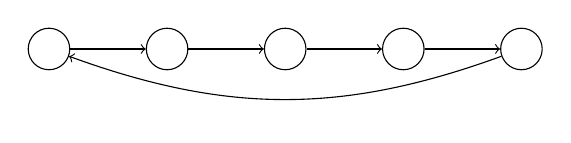
\begin{tikzpicture}
\tikzstyle{nodo} = [draw, circle, minimum size=1.5em]

\node[nodo] (A1) at (1,0) {};
\node[nodo] (A2) at (2.5,0) {};
\node[nodo] (A3) at (4,0) {};
\node[nodo] (A4) at (5.5,0) {};
\node[nodo] (A5) at (7,0) {};

\draw[->] (A1) -- (A2);
\draw[->] (A2) -- (A3);
\draw[->] (A3) -- (A4);
\draw[->] (A4) -- (A5);

\draw[->] (A5) edge [bend left=20] (A1);
\end{tikzpicture}
\caption{Anillo de procesos con $n=5$}
\label{fig:anillo}
\end{figure}

Para resolver este problema, se plantean tres comportamientos:

\begin{description}
 \item [Node] modela cada nodo del anillo.
 \item [Ring] espera un mensaje con una cantidad de nodos a crear, y una cantidad de mensajes a enviar.
 \item [BuildingRing] cumple la función de estructura de control, crea el anillo de nodos.
\end{description}

\subsubsection*{Comportamiento de Node}

\textbf{Node} reacciona entre dos comunicaciones diferentes: $'point\_to'$ y $'msg'$. En el caso de $'point\_to'$, cuando lo procesa, cambia al nodo que apunta. Cuando procesa un mensaje de tipo $['msg']$, siempre reenvía al siguiente nodo en la lista la comunicación $['msg']$. Si el valor del contador $m$ es mayor que cero, se disminuye el contador en uno y sigue con la ejecución. Si es cero, termina la ejecución en ese momento.

Código en \SAL para \textbf{Node}:

\begin{lstlisting}[language=sal, style=simple]
def Node(m, next) match
  case ['point_to', newNext]:
    become Node(m, newNext)
  case ['msg']:
    if ( m = 0 ) then
      send ['msg'] to next
    else
      send ['msg'] to next
      become Node(m - 1, next)
    end if
end def
\end{lstlisting}

Código en \CSP:

\begin{process}
Node(self, m, next) = \\ \quad
  \begin{block}
  CommRecv.self?\langle 'point\_to', newNext \rangle \then \\
  Node(self, m, newNext)
  \end{block} \\

  \Extchoice \\ \quad
  
  \begin{block}
  CommRecv.self?\langle 'msg' \rangle \then {} \\ \quad
    \begin{block}
    \If (m == 0) \Then {} \\ \quad
      \begin{block} 
      CommSend!next.\langle 'msg' \rangle \then \\
      STOP
      \end{block} \\
    \Else {} \\ \quad
      \begin{block}
      CommSend!next.\langle 'msg' \rangle \then \\
      Node(self, m - 1, next) 
      \end{block}
    \end{block}
  \end{block} 
\end{process}

% Donde:
% 
% \begin{description}
%  \item [Linea 2-3] Si responde a un mensaje de tipo $'point_to'$, el comportamiento de reemplazo es \textbf{Node} pero cambiando el parametro $next$ por $newNext$.
%  \item [Linea 4-5] Si responde a un mensaje de tipo $'msg'$, y su contador $m$ es mayor que cero, envia un mensaje al proximo actor el anillo ($next$). Su comportamiento de reemplazo es \textbf{Node} pero decrementando en uno el contador $m$.
%  \item [Linea 7] Si responde a un mensaje de tipo $'msg'$, y su contador $m$ era cero, envia un mensaje al proximo actor en el anillo ($next$). Como no define comportamiento de reemplazo, termina su ejecución en es momento.
% \end{description}

\subsubsection*{Comportamiento de Ring}

Cuando \textbf{Ring} recibe una comunicación con una lista que tiene un par de enteros, el primero de los enteros es la cantidad de nodos a crear, y el segundo es la cantidad de comunicaciones a mandar. Crea el primer nodo que va a tener el anillo y el actor que va a estar encargado de crear el resto del anillo. Le envía un mensaje a $builder$ con el número de nodos que tiene que crear. Como el primero fue inicialiado este es decrementado en uno.

Código en \SAL:

\begin{lstlisting}[language=sal, style=simple]
def Ring()[n, m]
  let first = new Node(m, nil)
      builder = new BuildingRing(first, first) 
  in
    send [n - 1, m] to builder
    become Ring() 
end def
\end{lstlisting}

Código en \CSP:

\begin{process}
Ring(self) = \\ \quad
  \begin{block}
  CommRecv.self?\langle n, m \rangle \then \\
  CreateAsk?node.first!\langle m, Null \rangle \then \\
  CreateAsk?buildingRing.builder!\langle node.first, node.first \rangle \then \\
  CommSend.buildingRing.builder!\langle n - 1, m\rangle \then \\
  Ring(self)
  \end{block}
\end{process}

\subsubsection*{Comportamiento de BuildingRing}

Esta es una estructura de control, siempre que procese una comunicación con $n$ mayor a uno, crea un nuevo nodo. Le envía al nodo que creó en la iteración anterior un mensaje para que apunte al nuevo nodo creado. Se auto enviá un mensaje decrementando en uno el contador de nodos a crear. El comportamiento de reemplazo cambia el nodo $lastCreated$.

Si el contador $n$ era cero, le envía un mensaje al nodo creado en la iteración anterior para que apunte al primer nodo creado ($first$). De esta manera cierra el anillo. Le envía una comunicación al primer nodo, que da inicio al envío de mensajes. 

Código en \SAL:

\begin{lstlisting}[language=sal, style=simple]
def BuildingRing(m, first, lastCreated)[n, m]
  if (n == 0) then
    send ['poins_to', first] to lastCreated,
    send ['msg'] to first
  else
    let newNode = new Node(m, null) in
      send ['point_to', newNode] to lastCreated
      send [ n - 1, m ] to self
      become BuildingRing(first, newNode)
  end if
end def
\end{lstlisting}

Código en \CSP:

\begin{process}
BuildingRing(self, first, lastCreated) = \\ \quad
  \begin{block}
  CommRecv.self?\langle n, m \rangle \then \\ \quad
  \begin{block} 
  \If (n == 0) \Then {} \\ \quad
    \begin{block}
    CommSend!lastCreated.\langle 'point\_to', first \rangle \then \\
    CommSend!first.\langle 'msg' \rangle \then \\
    STOP
    \end{block} \\
  \Else {} \\ \quad
    \begin{block} 
    CreateAsk?node.newNode!\langle m, Null \rangle \then \\
    CommSend!lastCreated.\langle 'point\_to', node.newNode \rangle \then \\
    CommSend!send.\langle n - 1, m \rangle \then \\
    BuildingRing(self, first, node.newNode) 
    \end{block} \\
  \end{block} 
\end{block}
\end{process}

\section{Una semántica en CSP}

En esta sección se describen cómo traducir las expresiones, los comandos y los comportamientos desde \SAL a \CSP. Para esto se utiliza la gramática definida en \ref{actores:sal}. Las funciones esta definidas de manera inductiva.

\subsubsection*{Expresiones}

En la sección \ref{actores:exp} se definió la gramática para las expresiones. Para traducir estas expresiones se utilizan las siguientes funciones:

La función $exp_{tr}$ viene dada de la siguiente forma:

\begin{equation*}
  exp_{tr}(exp) =
  \setlength{\arraycolsep}{0pt}
  \renewcommand{\arraystretch}{1.2}
  \left\{\begin{array}{l @{\quad} l}
        iexp_{tr}(exp)    & \text{cuando exp es de tipo iexp} \\
        bexp_{tr}(exp)    & \text{cuando exp es de tipo bexp} \\
        mexp_{tr}(exp)    & \text{cuando exp es de tipo mexp} \\
        sexp_{tr}(exp)    & \text{cuando exp es de tipo sexp} \\
  \end{array}\right.
\end{equation*}

La función para las expresiones de enteros, $iexp_{tr}$ viene dada de la siguiente forma:

\begin{equation*}
\begin{array}{l c l}
iexp_{tr}(iexp_1 + iexp_2) &=& iexp_{tr}(iexp_1) + iexp_{tr}(iexp_2) \\
iexp_{tr}(iexp_1 - iexp_2) &=& iexp_{tr}(iexp_1) - iexp_{tr}(iexp_2) \\
iexp_{tr}(iexp_1 * iexp_2) &=& iexp_{tr}(iexp_1) * iexp_{tr}(iexp_2) \\ 
iexp_{tr}(iexp_1 / iexp_2) &=& iexp_{tr}(iexp_1) / iexp_{tr}(iexp_2) \\
iexp_{tr}(- iexp) &=& - iexp_{tr}(iexp)
\end{array}
\end{equation*}

La función expresiones booleanas $bexp_{tr}$ es finalmente:

\begin{equation*}
\begin{array}{l c l}
bexp_{tr}(bexp_1 \textbf{ or } bexp_2) &=& bexp_{tr}(iexp_1) \vee bexp_{tr}(iexp_2) \\
bexp_{tr}(bexp_1 \textbf{ and } bexp_2) &=& bexp_{tr}(iexp_1) \wedge bexp_{tr}(iexp_2) \\
bexp_{tr}(\textbf{not } bexp) &=& \neg bexp_{tr}(bexp) \\ 
bexp_{tr}(exp_1 == iexp_2) &=& exp_{tr}(exp_1) == exp_{tr}(exp_2) \\
\end{array}
\end{equation*}

Tanto $mexp_{tr}$ como $sexp_{tr}$ no tienen una traducción asociada, podrían definirse como la función identidad.

\subsubsection*{Comportamientos}
En la sección \ref{actores:beha} se definió la gramática para las expresiones. Para traducir estas expresiones se utilizan las funciones $beha_{tr}$ y $body_{tr}$.

La función $beha_{tr}$ viene dada por la forma:

\begin{multline*}
beha_{tr}(\textbf{def } BehName(p_1, p_2,\ldots, p_n)\ body \textbf{ end def}) = \\
BehName(self, p_1, p_2,\ldots, p_n) = body_{tr}(body) 
\end{multline*}

La función $body_{tr}$ viene dada por la forma:

\begin{multline*}
body_{tr}([ p_1, p_2,\ldots, p_n]\ command) = \\
 CommRecv.self?\langle p_1, p_2,\ldots, p_n \rangle \then cmd_{tr}(command)
\end{multline*}

\begin{multline*}
body_{tr}(\textbf{ case } [p_{11}, p_{12},\ldots, p_{1n}]: command_1 \ldots \textbf{ case } [p_{n1}, p_{n2},\ldots, p_{nk}]: command_n ) = \\
CommRecv.self?\langle p_{11}, p_{12},\ldots, p_{1n} \rangle \then cmd_{tr}(command_1) \ldots \\
\Extchoice CommRecv.self?\langle p_{n1}, p_{n2},\ldots, p_{nk} \rangle \then cmd_{tr}(command_n) 
\end{multline*}

\subsubsection*{Comandos}

En la sección \ref{actores:cmd} se definió la gramática para los comandos. Para traducir los comandos se utiliza la función $cmd_{tr}$, que se define de la siguiente forma:

\begin{multline*}
cmd_{tr} (\textbf{send } exp_1, exp_2, \ldots\ , exp_n \textbf{to } mexp) = \\
CommSend.mexp. \langle exp_{tr}(exp_1), exp_{tr}(exp_2), \ldots, exp_{tr}(exp_m) \rangle
\end{multline*}

\begin{multline*}
cmd_{tr} (\textbf{become}\ B(exp_1, exp_2,\ \ldots, exp_n)) = \\
B(exp_{tr}(exp_1), exp_{tr}(exp_2), \ldots, exp_{tr}(exp_n)) \rangle
\end{multline*}

\begin{multline*}
cmd_{tr} (command_1 \textbf{;} command_2) = cmd_{tr}(command_1) \then cmd_{tr}(command_2)
\end{multline*}

\begin{multline*}
cmd_{tr} (\textbf{if } bexp \textbf{ then } command_1 \textbf{ else } command_2 \textbf{ end if }) = \\
\textbf{if } (bexp_{tr}(bexp))\textbf{ then } cmd_{tr}(command_1) \textbf{ else } cmd_{tr}(command_2)
\end{multline*}

\begin{multline*}
cmd_{tr}( \textbf{let}\ mexp_1 = \textbf{new} B_1(exp_{11}, exp_{12},\ \ldots, exp_{1m}), \ldots, \\
mexp_n = \textbf{ new }B_n(exp_{n1}, exp_{n2},\ldots, exp_{nk}) \textbf{ in }command) = \\
CreateAsk?b_1.pid_1! \langle exp_{tr}(exp_{11}), exp_{tr}(exp_{12}),\ \ldots, exp_{tr}(exp_{1m}) \rangle \then \ldots \\
CreateAsk?b_N.pid_n! \langle exp_{tr}(exp_{n1}), exp_{tr}(exp_{n2}),\ \ldots, exp_{tr}(exp_{nk}) \rangle \then  \\ 
cmd_{tr}(command)
\end{multline*}

\subsubsection*{Pasos finales}

El sistema final cuenta de todos los componentes del sistema de actores en paralelo. Estos componentes son: los buzones vistos en la sección \ref{modelo:buzon}, los procesos que separan la intención de crear de la creación propiamente dicha vistos en la sección \ref{modelo:crear} y los preámbulos vistos en la misma sección.

La comunicación va desde estos preámbulos hacia los buzones. Los eventos de interés en este caso son todos los generados por los buzones. Es decir el conjunto generado $CommSend.i.j$ donde $i$ son todos los posibles actores e $j$ son las mensajes a enviar. A estos eventos se le debe unir el conjunto generado por los eventos $CommRecv.i.j$ donde $i$ son todos los posibles actores y $j$ son las mensajes a enviar. Este es el conjunto de todas los eventos posible de loa buzones. Este conjunto se denomina: $Comm$.

Otra forma de comunicación es desde estos preámbulos hacia los procesos que separan la intención de crear a la creación, Es decir el conjunto generado por $CreateAsk.i.j$ donde $i$ son todos los posibles actores y $j$ son todos los posibles valores de \textit{acquaiantence-list}. A estos eventos se le debe unir el conjunto generador por $Create.i.j$ donde $i$ son todos los posibles actores y $j$ son todos los posibles valores de \textit{acquaiantence-list}. Este conjunto se denomina $Init$.

Ahora suponiendo que tenemos dos conjunto de actores $ks$ y $js$ definidos a continuación.

\begin{align*}
ks = \Interleave_{ self : ACTOR_k } & Create!self?<p1, p2> \then \\
& K(self, p1, p2)  \\ 
js = \Interleave_{ self : ACTOR_j } & Create!self?<p1, p2> \then \\
& J(self, p1, p2) 
\end{align*}

donde $J$ y $K$ son dos definiciones de comportamiento. Para integrar todo el sistema de actores tendríamos que escribir la siguiente ecuación:

\begin{align*}
SYSTEM =  (ks \Interleave js) \Parallel\limits_{Comm \cup Init} (Mailboxes \Interleave Creates)
\end{align*}

Donde $Mailboxes$ está definido en la sección \ref{modelo:buzon} y $Creates$ en la sección \ref{modelo:crear}. Entre $ks$ y $js$ nunca existe ningún tipo de comunicación, por eso se usa el operador de entrelazado. Lo mismo ocurre con $Mailboxes$ y $Creates$.

\section{Corriendo los modelos en FDR}

Esta sección muestra algunas modificaciones necesarias que fueron hechas al modelo para poderlo correr utilizando \FDR. \FDR es un verificador de refinamiento para \CSP. Permite definir procesos de \CSP utilizando el lenguaje \CSPm. Se pueden verificar varias afirmaciones sobre estos procesos. A continuación se cuentan algunas de estas características.

\textit{probe} puede utilizarse para explorar manualmente las transiciones de un proceso como si fuera un árbol, es muy útil para al depurar una definición de proceso. Esto fue particularmente útil al explorar la creación del modelo antes propuesto. Se mostrará un caso donde se puede ver el gráfico de todas las ejecuciones de uno de los ejemplos. 
 
También es posible verificar refinamiento utilizando el modelo de trazas o el modelo divergencias. Se verá un ejemplo de como es posible verificar este tipo de afirmaciones.

Esta son algunas de las posibles pruebas que se pueden hacer utilizando la herramienta, pero no son exhaustivas. Para mayor información sobre la herramienta se puede consultar su manual\cite{fdrmanual}.

\subsection{Restricciones sobre el modelo}

Es necesario imponer restricciones al utilizar \FDR. Estas restricciones están relacionas a cómo la herramienta explora los estados posibles del modelo. Por ejemplo, si se utiliza el rango completo de enteros intentará revisar cada uno de estos enteros, haciendo cada exploración exponencial en cada estado que se visite. En el resto de esta sección se exploran estas restricciones. Las modificaciones que incluyen estas restricciones pueden verse en los ejemplos en el apéndice \ref{codigo}.

\subsubsection*{Enteros pequeños}

Para evitar la explosión de estados que causa utilizar el rango de enteros de \textit{64-bits}, se genera una una representación propia para reducirla. Para esto se utiliza un tipo algebraico que representa estos enteros:

\begin{align*}
datatype\ SmallInt =&\ SI.\{0 \ldots MAX\_INT\} | Overflow \\
\end{align*}

Donde, $MAX\_INT$ es el entero más grande que se quisiera representar. Aparte de esta representación de los enteros, se construyeron las operaciones básicas sobre ellos:

\begin{align*}
add(SI.a, SI.b)\ =&\ let\ sum\ = a + b \\
&within\ if\ sum <= MAX\_INT\ then\ SI.sum\ else\ Overflow  \\
%
sub(SI.a, SI.b) =&\ let\ sub\ =\ a - b \\
& within\ if\ sub >= 0\ then\ SI.sub\ else\ Overflow \\
%
mult(SI.a, SI.b) =&\ let\ mult\ = a * b \\
& within\ if\ mult <= MAX\_INT\ then\ SI.mult\ else\ Overflow \\
eq(SI.a, SI.b)\ =&\ a == b \\
eq(\_, \_)\ =&\ false
\end{align*}

Donde $add$ es la suma, $sub$ la resta, $mult$ la multiplicación y $eq$ la igualdad. Si alguna operación excede el entero máximo el resultado de esta es $Overflow$.

\subsubsection*{Listas de parámetros y valores}
En en modelo se utilizan listas para representar tanto los parámetros de \textit{acquaiantence-list} y los de \textit{communication-list}. Las listas son potencialmente infinitas, pare evitar que el modelo explore todos estos estados, se limita el tamaño de las listas. Se utilizan tuplas de tamaño fijo. Para esto es necesario conocer el tamaño máximo del mensaje que se va a enviar, esta es una limitación del modelo presentado.

La expresividad de los mensajes es grande. Un actor podría recibir un mensaje del tipo $['transferir', buz\acute{o}n_1, buz\acute{o}n_2]$, donde el primer buzón representa la caja de ahorro origen y el segundo la de destino. El siguiente mensaje que procese el mismo actor podría ser $['depositar', monto, buz\acute{o}n]$ donde monto es un entero con el monto a depositar y el buzón representa la caja de ahorro a la cual depositar. 

Para poder tener cierta flexibilidad en el momento de enviar mensajes, se creá una unión de tipos llamada $VALUE$. Este tipo codifica todos los posibles valores que se quisieran enviar, buzones, enteros, booleanos y cadenas. Como las tuplas se definen de tamaño fijo, es necesario agregar un tipo con la funcionalidad de marcar la posición. Esto funciona de la siguiente manera: si las listas son de tamaño tres, no necesariamente todos los mensajes son de esta longitud, podría existir un mensaje que sea una lista de tamaño dos, por ejemplo: $[1, client]$. La tupla de tamaño tres sería $(1, None, None)$. Se define $VALUE$ de la siguiente forma:

\[
  datatype\ VALUE = ACTOR.ActorID | INT.SmallInt | BOOL.Bool | ATOM.Atoms | None
\]

Las cadenas de caracteres se representa utilizando $Atoms$. Las cadenas son inmutables y la única operación que se efectúa sobre ellas es la comparación. La definición de $Atoms$ viene dada de la siguiente forma:

\[
  datatype\ Atoms = ATOM_1 | ATOM_2 | \ldots | ATOM_n
\]

\subsubsection*{Cota en el buzón}

Se puede modelar un buzón que no tenga una cota superior, pero se tendría nuevamente problemas de explosión de estados ya que \FDR intentaría explorar todas las combinaciones posibles de buzón. Este caso es similar al de la lista en la comunicación. 

La ecuación de \textit{buzón}, con cota, es la siguiente:

\begin{process}

\begin{block}
MAILBOX\_SIZE = 4
\end{block} \\

\begin{block}
Mailbox(i, \nil) = {} \\ \quad
CommSend?i.x \then Mailbox(i, \lseq x \rseq) 
\end{block} \\

\begin{block}
Mailbox(i, msgs) = {} \\ \quad
  \begin{block} 
  \If (length(msgs) < MAILBOX\_SIZE - 1) \Then {} \\ \quad
    \begin{block} 
      MailboxWithSpace(i, msgs)
    \end{block} \\
  \Else {} \\ \quad
    \begin{block}
      MailboxFull(i, msgs)
    \end{block}
  \end{block} 
\end{block} \\

\begin{block}
MailboxWithSpace(i, \lseq x \rseq \cat xs ) = {} \\ \quad 
  \begin{block}
    CommRecv!i.x \then Mailbox(i, xs) \\
    \Extchoice \\
    CommSend?i.y \then Mailbox(i, \lseq x \rseq \cat xs \cat \lseq y \rseq ) 
  \end{block}
\end{block} \\

\begin{block}
MailboxFull(i, \lseq x \rseq \cat xs ) = {} \\ \quad 
  \begin{block}
    CommRecv!i.x \then Mailbox(i, xs) \\
  \end{block}
\end{block} \\
\end{process}

La ecuación anterior le agrega a la vista en la sección \ref{modelo:buzon}, un límite definido por $MAILBOX\_SIZE$. El comportamiento del proceso buzón depende de su estado, si no tiene ningún mensaje, o si tiene al menos algún mensaje o si está completo.

\begin{itemize}
\item Si no tiene ningún mensaje, solo sincroniza mensajes por el canal $CommSend$.
\item Si tiene algunos mensajes, por los canales $CommSend$ y $CommRecv$.
\item Si llegó a su capacidad máxima $MAILBOX\_SIZE$ lo hace solo por el canal $CommRecv$.
\end{itemize}

\subsection{Algunos resultados}

A continuación se muestran dos resultados obtenidos utilizando el modelo propuesto en \CSP. Uno explora el gráfico de entrelazado y el otro verifica una afirmación utilizando el modelo de trazas.

\subsubsection*{Gráfico de interacciones}

Utilizando la función \textit{probe} de la herramienta \FDR, se puede ver permite ver gráfico de interacciones de los distintos procesos. En el caso del modelo, permite ver como las diferentes interacciones de los actores.

\begin{figure}[H]

\begin{center}
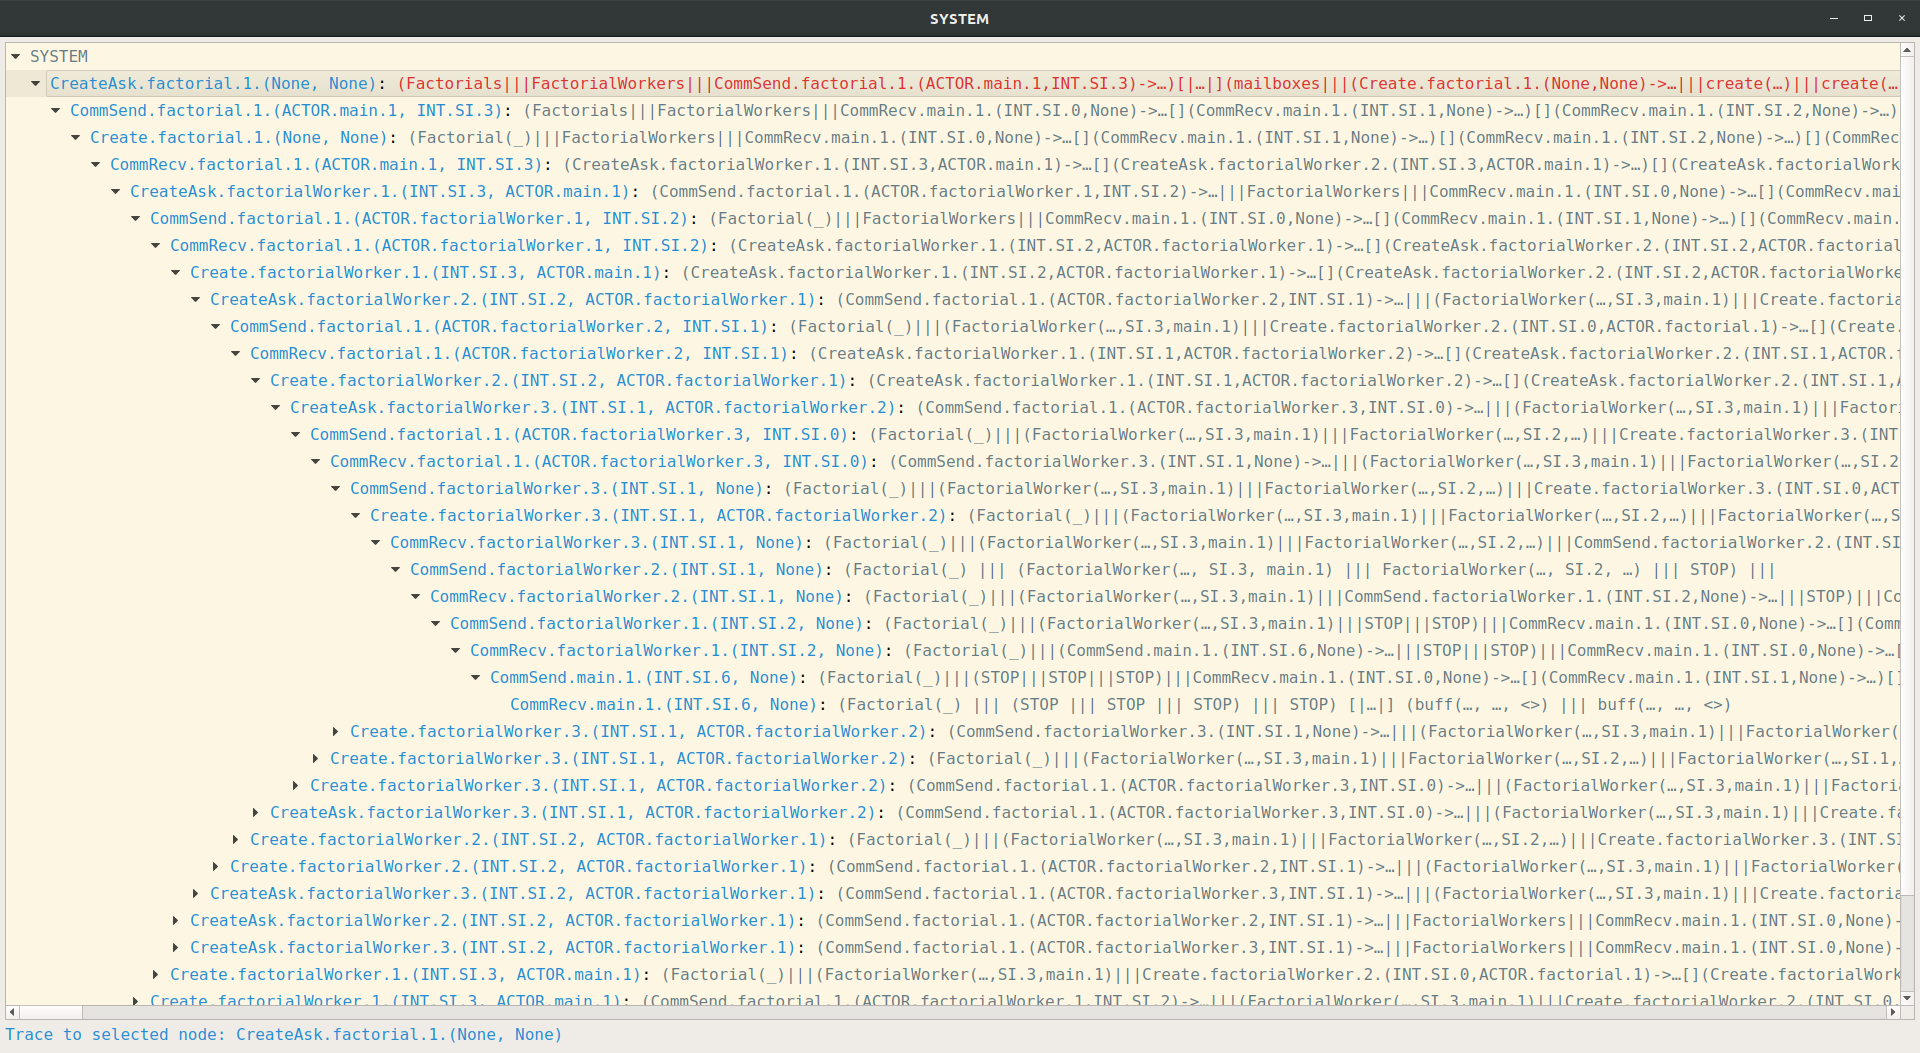
\includegraphics[width=15 cm]{img/fact.png}
\caption{Calculo del factorial de 3 visto en \ref{fig:factorial}}\label{modelo:grafo}
\end{center}
\end{figure}

Se pueden ver en la figura \ref{modelo:grafo} las siguientes acciones:

\begin{itemize}
\item $Main$ crea un actor con el comportamiento $Factorial$
\item $Main$ le envía a $Factorial$, un mensaje con su dirección de buzón y el número 3.
\item Se crea el actor $Factorial$
\item $Factorial$ recibe el mensaje con la dirección de $Main$ y el número 3.

\item $Factorial$ crea un actor de tipo $FactorialWorker$ ($factorialWorker_1$). Está inicializado con los parámetros: el entero 3, y el buzón del actor $Main$.
\item $Factorial$ se auto envía el mensaje con el valor 2 y la dirección de buzón de $factorialWorker_1$.
\item $Factorial$ recibe el mensaje con la dirección de $factorialWorker_1$ y el número 2.
\item Se crea el actor $FactorialWorker$ con buzón $factorialWorker_1$.

\item $Factorial$ crea un actor de tipo $FactorialWorker$ ($factorialWorker_2$). Está inicializado con los parámetros: el entero 3, y el buzón del actor $factorialWorker_1$.
\item $Factorial$ se auto envía el mensaje con el valor 1 y la dirección de buzón de $factorialWorker_2$.
\item $Factorial$ recibe el mensaje con la dirección de $factorialWorker_2$ y el número 1.
\item Se crea el actor $FactorialWorker$ con buzón $factorialWorker_2$.

\item $Factorial$ crea un actor de tipo $FactorialWorker$ ($factorialWorker_3$). Está inicializado con los parámetros: el entero 1, y el buzón del actor $factorialWorker_2$.
\item $Factorial$ se auto envía el mensaje con el valor 0 y la dirección de buzón de $factorialWorker_3$.
\item $Factorial$ recibe el mensaje con la dirección de $factorialWorker_3$ y el número 0.
\item Se crea el actor $FactorialWorker$ con buzón $factorialWorker_3$.

\item $Factorial$ le envía a $factorialWorker_3$ el entero 1.
\item $factorialWorker_3$ recibe el valor 1.

\item $factorialWorker_3$ le envía a $factorialWorker_2$ el entero 1.
\item $factorialWorker_2$ recibe el valor 1.

\item $factorialWorker_2$ le envía a $factorialWorker_1$ el entero 2.
\item $factorialWorker_1$ recibe el valor 2.

\item $factorialWorker_1$ le envía a $Main$ el entero 6.
\item $Main$ recibe el valor 6.

\end{itemize}

Esta captura fue realizada utilizando el comando \verb=:probe SYSTEM= en \FDR en el código de factorial del apéndice \ref{codigo:factorial}.

\subsubsection*{Refinamiento}

En \FDR para probar si un proceso P refina en proceso Q se escribe \verb$assert P [T= Q$. En esta prueba de refinamiento, se utilizó el ejemplo de la cola visto en la sección \ref{ejemplo:cola}. El código \CSPm se encuentra en el apéndice \ref{codigo:cola}.

Dado dos actores ``main'', \verb=actor_main1= y \verb=actor_main2=:

\begin{verbatim}
actor_main1 = CreateAsk?queue.pid!(None, None) ->
              actor_main1_r(queue.pid)

actor_main1_r(pid) =
    CommSend.pid!(ATOM.ENQUEUE, INT.SI.1) -> 
    actor_main1_r(pid) 
    |~| 
    CommSend.pid!(ATOM.ENQUEUE, INT.SI.2) -> 
    actor_main1_r(pid)
    |~| 
    CommSend.pid!(ATOM.DEQUEUE, ACTOR.main.1) -> 
    CommRecv.main.1?(INT.V, None) -> 
    actor_main1_r(pid)

\end{verbatim}
Donde el actor \verb=actor_main1=, después de crear un actor \textit{Queue}, hace uso de la selección externa para:
\begin{itemize}
 \item enviar a el actor \textit{Queue} un mensaje $['enqueue', 1]$
 \item enviar a el actor \textit{Queue} un mensaje $['enqueue', 2]$
 \item enviar a el actor \textit{Queue} un mensaje $['dequeue', buzonDeMain]$, seguido de esperar recibir un entero.
\end{itemize}

\begin{verbatim}

actor_main2 = CreateAsk?queue.pid!(None, None) ->
              actor_main2_r(queue.pid)

actor_main2_r(pid) =
      CommSend.pid!(ATOM.ENQUEUE, INT.SI.1) -> 
      CommSend.pid!(ATOM.ENQUEUE, INT.SI.2) -> 
      actor_main2_r(pid) 
      |~|
      CommSend.pid!(ATOM.DEQUEUE, ACTOR.main.1) -> 
      CommRecv.main.1?(INT.V, None) -> 
      actor_main2_r(pid)
\end{verbatim}

Donde el actor \verb=actor_main2=, después de crear un actor \textit{Queue}, hace uso de la selección externa para:
\begin{itemize}
 \item enviar a el actor \textit{Queue} un mensaje $['enqueue', 1]$, seguido de enviar a el actor \textit{Queue} un mensaje $['enqueue', 2]$
 \item enviar a el actor \textit{Queue} un mensaje $['dequeue', buzonDeMain]$, seguido de esperar recibir un entero.
\end{itemize}

El resultado de poner en paralelo todos los componentes del sistema utilizando \verb=actor_main1= se llama \verb=SYSTEM1=. En el caso de \verb=actor_main2= se llama \verb=SYSTEM2=.

\begin{figure}[H]
\begin{center}
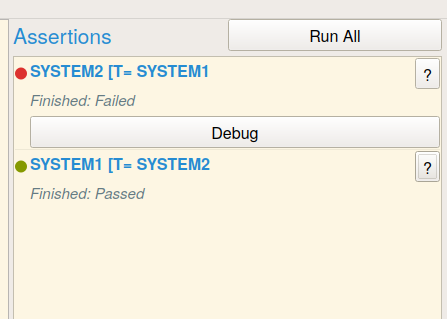
\includegraphics[width=5 cm]{img/trazas.png}
\caption{Resultado de las afirmaciones}\label{modelo:verifica}
\end{center}
\end{figure}

Para probar si $SYSTEM1$, refina en $SYSTEM2$ se utiliza la siguiente afirmación:

\begin{verbatim}
assert SYSTEM1 [T= SYSTEM2 
\end{verbatim}

Para probar si $SYSTEM2$, refina en $SYSTEM1$ se utiliza la siguiente afirmación:

\begin{verbatim}
assert SYSTEM2 [T= SYSTEM1 
\end{verbatim}

Puede verse en la figura \ref{modelo:verifica} el resultado de correr ambas afirmaciones. Utilizando la herramienta se encuentra un contraejemplo donde  SYSTEM2 no refina en SYSTEM1 como muestra la figura \ref{modelo:contraejemplo}.
 

\begin{figure}[H]
\begin{center}
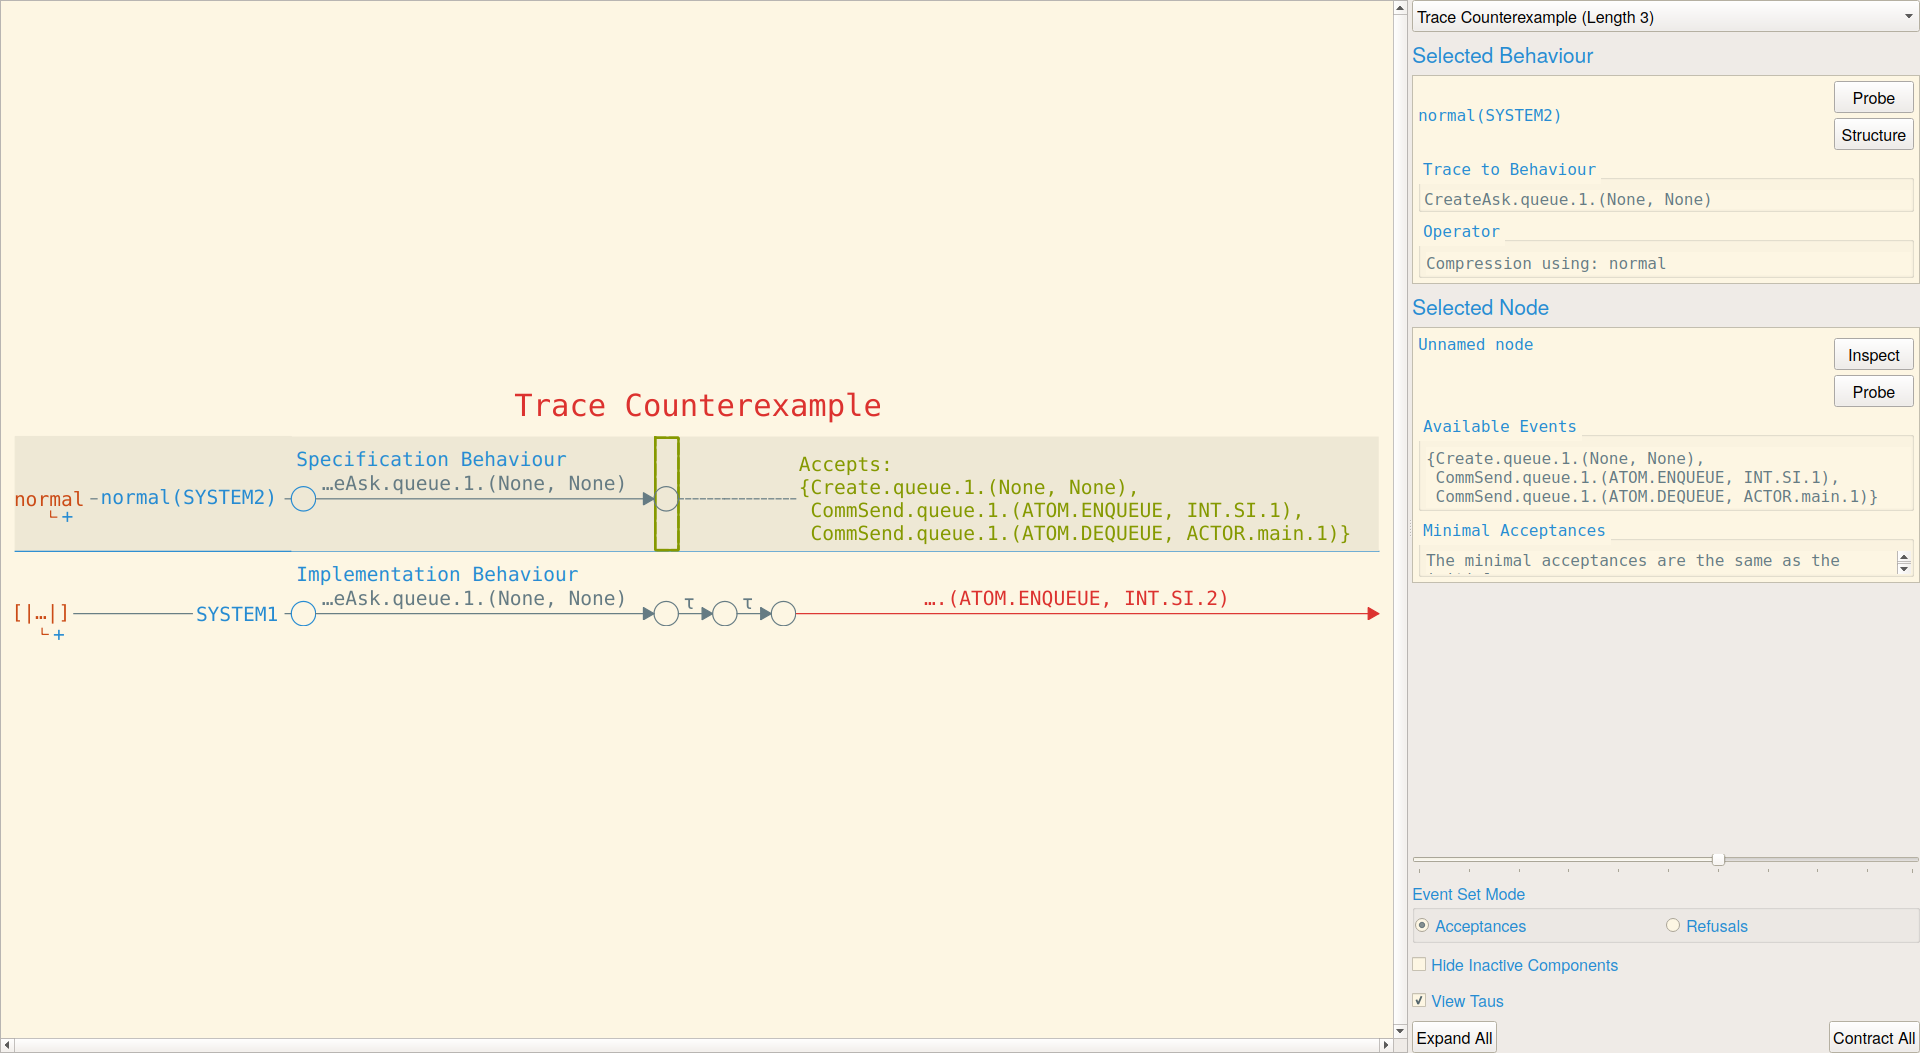
\includegraphics[width=15 cm]{img/contraejemplo.png}
\caption{Contraejemplo de SYSTEM2 refina en  SYSTEM1}\label{modelo:contraejemplo}
\end{center}
\end{figure}
 
